\documentclass{article}
\usepackage[a4paper,]{geometry}
\usepackage{lmodern}
%\usepackage[export]{adjustbox}
\usepackage[utf8]{inputenc}
\usepackage[T1]{fontenc}
\usepackage{graphicx}
%\usepackage{titlepic}
\usepackage{mathtools}
%\usepackage{amsmath}
%\usepackage{amssymb}
%\usepackage{amsfonts}
\usepackage{wasysym}
%\usepackage{accents}
%\usepackage{esvect}
%\usepackage{subcaption}
\usepackage{multicol}
\usepackage{hyperref}
%\usepackage{enumitem}
\usepackage[makeroom]{cancel}
\usepackage{siunitx}
\usepackage{float}
\usepackage{lipsum}
\usepackage{textcomp}
\usepackage{circuitikz}
\usepackage{placeins}

\sisetup{separate-uncertainty=true}
\linespread{1.3}

% my commands
\newcommand{\E}[1]{\, \mathrm{e}{#1} \, }
\newcommand{\de}{\mathrm{d}}
\newcommand{\pars}{\mathbin{\!/\mkern-5mu/\!}}
\newcommand{\equalexpl}[1]{
	\underset{\substack{\uparrow\\\mathrlap{\text{#1}}}}{=}}

% circuits stuff
\tikzset{
  declare function={% in case of CVS which switches the arguments of atan2
    atan3(\a,\b)=ifthenelse(atan2(0,1)==90, atan2(\a,\b), atan2(\b,\a));},
  kinky cross radius/.initial=+.125cm,
  @kinky cross/.initial=+, kinky crosses/.is choice,
  kinky crosses/left/.style={@kinky cross=-},kinky crosses/right/.style={@kinky cross=+},
  kinky cross/.style args={(#1)--(#2)}{
    to path={
      let \p{@kc@}=($(\tikztotarget)-(\tikztostart)$),
          \n{@kc@}={atan3(\p{@kc@})+180} in
      -- ($(intersection of \tikztostart--{\tikztotarget} and #1--#2)!%
             \pgfkeysvalueof{/tikz/kinky cross radius}!(\tikztostart)$)
      arc [ radius     =\pgfkeysvalueof{/tikz/kinky cross radius},
            start angle=\n{@kc@},
            delta angle=\pgfkeysvalueof{/tikz/@kinky cross}180 ]
      -- (\tikztotarget)}}}



\title{Diodi}
%\subtitle{Caratteristiche e ponte di Graetz}
\author{Filippo Dal Farra \and Matteo Zandegiacomo Orsolina}
\date{Gennaio 2018}

\begin{document}

\maketitle

\newpage

\section{Introduzione}

Nel corso di questa esperienza ci siamo interessati allo studio dei diodi, i quali sono elementi di circuito non lineari dotati di alcune proprietà che abbiamo avuto modo di osservare. Essi sono composti da una giunzione P-N, il che li rende degli elementi asimmetrici. Di conseguenza se messi in un senso piuttosto che nell'altro si comportano in modo diverso: in un caso permettono il passaggio di corrente, nell'altro la interdicono. 
%non vuol dire un cazzo di niente: Si prende un diodo posto nella direzione che permette ad $i$ di scorrere. 
In base alle loro caratteristiche sono stati creati dei modelli che affermano che corrente che la caduta di potenziale $\Delta V$ da essi prodotta \'e approssimativamente costante in funzione di $i$, una volta che si è superato un certo valore di soglia.\\ 

Nel prosieguo dell'esperienza sono stati introdotti anche i diodi Zener, il cui comportamento risulta simile ai diodi normali sotto certi aspetti, ma di gran lunga diverso per altri. Il diodo Zener infatti permette sia una polarizzazione diretta che una inversa. Garantisce cioè una $\Delta V$ molto stabile attorno ad un particolare valore ($5.1\ \si{\volt}$ nel nostro caso) qualunque sia $i$ che gli scorre attraverso. \\
Questi elementi sono stati usati nel corso di questa esperienza per costruire un ponte di Graetz (altrimenti detto raddrizzatore ad onda intera). Si tratta di un rettificatore che poi \'e stato stabilizzato con filtro capacitivo e regolatore a diodo Zener. Infatti vengono sfruttati i diodi per rendere continua e stabile la tensione di alimentazione alternata.

\section{Materiali e strumenti}

\begin{itemize}
  \item 4 diodi 1N4007
  \item Un diodo Zener BZX85C 5V1 
  \item Multimetro digitale (DMM)
  \item Trasformatore step-down $\SI{220}{\volt}$ - $\SI{7.5}{\volt}$
  \item Tester analogico (ICE)
  \item Generatore di tensione variabile
  \item Un condensatore elettrolitico $\SI{200}{\micro\farad}$
  \item Resistenze varie
  \item Oscilloscopio
  \item Breadboard
  \item Cavi "banana-banana"
  \item Decade di resistenze
\end{itemize}

\section{Procedure di misura}

Per prima cosa abbiamo costruito un semplice circuito di misura con amperometro monte e alimentato dal generatore di tensione DC variabile. Abbiamo fatto ciò semplicemente per poterne studiare le caratteristiche e la sua relativa curva $i-V$, in polarizzazione diretta. Abbiamo adottato misure di $i$ comprese fra gli $1mA$ e i $300mA$ distribuite esponenzialmente. Per effettuare le misure \'e stato sfruttato in contemporanea DMM e tester ICE. Il primo ci è servito per misurare la $\Delta V$ ai capi del del diodo preso in considerazione, mentre il secondo lo abbiamo utilizzato per avere una misura di $i$ che passa attraverso di esso. Abbiamo ripetuto questa stessa operazione con quattro diodi diversi, sebbene solo su uno di essi abbiamo deciso di prendere un numero elevato di valori. \\

Abbiamo seguito lo stesso procedimento anche con un diodo Zener, questa volta però in polarizzazione inversa, poiché gli è permesso dalle sue caratteristiche fisiche sopra spiegate. In questo caso abbiamo scelto valori di corrente compresi tra $1mA$ e $150mA$. \'E stato alimentato il circuito con il generatore DC e per effettuare le misure abbiamo nuovamente sfruttato ICE e DMM. \\

Nella seconda parte dell'esperienza \'e stato costruito un ponte di Graetz in uscita al secondario di un trasformatore step-down a presa centrale (di cui \'e stata presa solo una met\'a) da $\SI{200}{\volt}$ a $\SI{7.5}{\volt}$ secondo in circuito in fig. \ref{fig:brid_cfilter}. Le misure di tensione sul carico sono state prese con il DMM e l'oscilloscopio in funzione del carico applicato tramite la decade di resistenze da $\SI{100}{\ohm}$ a circuito aperto.

\'E stato poi applicato l'ulteriore stadio di filtering con il diodo Zener secondo il circuito \ref{fig:bridgez} e le misurazioni sono state effettuate nuovamente.

\newpage

%%%%%%%%%%%%% ANAL-isis %%%%%%%%%%%%%%%%%%%
\section{Analisi dei dati}

L'esperienza è stata divisa in due parti: nella prima sono state studiate le caratteristiche di alcuni diodi rettificatori e di un diodo Zener, nella seconda invece ciò è stato applicato allo studio del ponte di Graetz.

\subsection{Diodi} 
L'esperienza è cominciata con lo studio del comportamento di alcuni diodi, sfruttando il circuito \ref{fig:cD}.

\begin{figure}[h]
    \begin{center}
    \begin{circuitikz} []
    \draw
        (0,2) to [battery] (0,0)
        (0,0) to (3,0)
        (0,2) to [ammeter] (2,2) 
        (2,2) to [Do] (2,0)
        (2,2) to (3,2)
        (3,2) to [open, *-*] (3,0);
    \end{circuitikz}
    \caption{Circuito usato per l'analisi dei diodi}
    \label{fig:cD}
    \end{center}
\end{figure}

Per ognuno dei quattro diodi a nostra disposizione abbiamo preso le misure di come varia $i$ in funzione di $\Delta V$. Qui esponiamo solo i dati di uno dei diodi, per evitare di ripetere sempre le stesse cose. I valori che otteniamo rappresentano una curva che assomiglia ad un'esponenziale, per cui proviamo a linearizzare il grafico. Ciò che otteniamo sono i due grafici riprodotti in figura \ref{fig:gDe} e \ref{fig:gDl}. 

\begin{figure}
    \centering
    \begin{minipage}{0.5\textwidth}
        \centering
        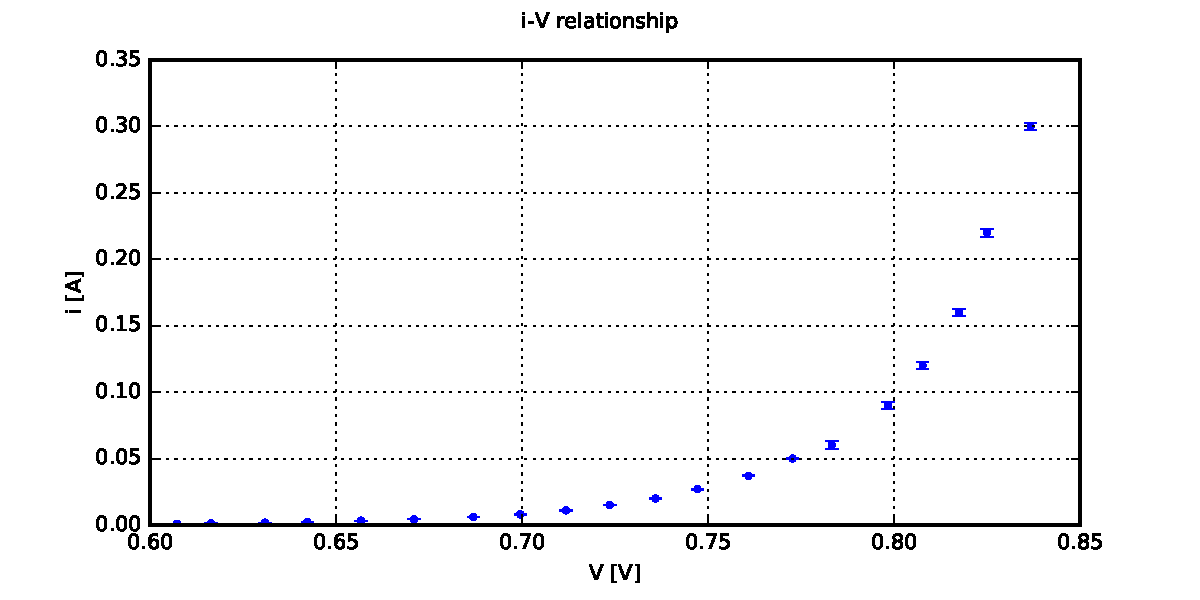
\includegraphics[width=\textwidth]{fig1D.pdf} 
        \caption{Grafico esponenziale di $i$ in funzione di $\Delta V$}
        \label{fig:gDe}
    \end{minipage}\hfill
    \begin{minipage}{0.5\textwidth}
        \centering
        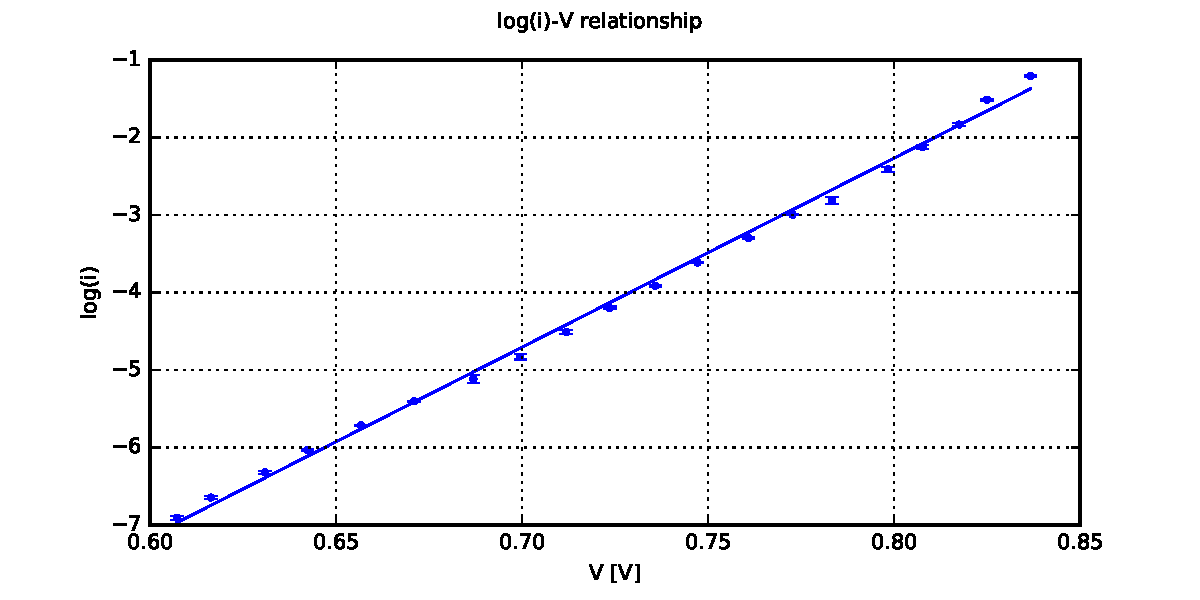
\includegraphics[width=\textwidth]{fig2D.pdf} 
        \caption{Grafico linearizzato di $\ln{i}$ in funzione di $\Delta V$ con relativo modello}
        \label{fig:gDl}
    \end{minipage}
    
\end{figure}
    
Proviamo quindi a cercare i parametri della retta ottenuta linearizzando il grafico attraverso una regressione lineare. Assumiamo che l'incertezza di $\Delta V$, cioè dovuta al DMM sia nulla. Mentre per trovare l'incertezza su $i$, $\sigma[i]$, assumiamo che all'interno dell'intervallo di incertezza massimo ci sia equiprobabilità tra tutti i possibili valori, per cui non possiamo sapere niente. Ovviamente quindi a seconda del fondo scala preso in considerazione varia l'incertezza sulla misura, che sarà cioè maggiore per i valori aventi una corrente più elevata. Per ottenere i valori di intercetta e pendenza prendiamo il grafico di $\Delta V$ in funzione di $i$, e a partire da esso quello di $\Delta V$ in funzione di $\ln{i}$. Attraverso il metodo dei minimi quadrati troviamo ora i valori di intercetta e pendenza di questo grafico, che chiameremo $A_p$ e $B_p$ rispettivamente. Ora non ci resta che invertire gli assi e propagare le incertezze sui nuovi parametri della retta e otteniamo il modello che descrive l'andamento, con dei valori $A$ e $B$ definitivi. \\

\begin{gather}
    \sigma[V]=0 \quad \sigma[i]= \frac{I_{FS}}{50 \sqrt{12}} \quad \sigma[\ln{i}] = \frac{\sigma[i]}{i}
    \\
    B = \frac{1}{B_p} = 24 \quad A = - A_p B = -21.8
    \\
    \sigma[B] = \frac{\sigma[B_p]}{B_p^2} = 1 \quad \sigma[A] = \sqrt{(B \sigma[A_p])^2 + (A_p \sigma[B])^2} = 0.9
    \\
    \label{eq:regr1}
\end{gather}

A parte qualche punto che si discosta un po' più degli altri osserviamo quindi che il modello descrive abbastanza bene i dati ottenuti. Infatti tutti i punti rientrano entro al massimo un $3\sigma$ dal modello, a parte solo l'ultimo. Perciò i valori di $i$ in funzione di $\Delta V$ seguono effettivamente un andamento esponenziale. \\
Un risultato analogo si è ottenuto anche per gli altri tre diodi da noi studiati. \\ \\

Consideriamo ora il diodo Zener, e studiamo il suo comportamento in modo analogo a quanto fatto con i diodi, sebbene con le dovute dovute alle differenti modalità di misura da noi adottate. In particolare il circuito da noi considerato è quello rappresentato in figura \ref{fig:cZ}

\begin{figure}[h]
    \begin{center}
    \begin{circuitikz} []
    \draw
        (0,2) to [battery] (0,0)
        (0,0) to (3,0)
        (0,2) to [ammeter] (2,2) 
        (2,0) to [zzDo] (2,2)
        (2,2) to (3,2)
        (3,2) to [open, *-*] (3,0);
    \end{circuitikz}
    \caption{Circuito usato per l'analisi dei diodi Zener}
    \label{fig:cZ}
    \end{center}
\end{figure}

Anche in questo caso studiamo $i$ in funzione di $\Delta V$ e ancora usiamo le stesse modalità per trovare i valori a cui siamo interessati. I calcoli sono li stessi di prima, perciò qui forniamo solo i risultati numerici.

\begin{gather}
    B = 4.30 \quad A = -25.3
    \\
    \sigma[B] = 0.04 \quad \sigma[A] = 0.3
    \\
    \label{eq:regr2}
\end{gather}

Andiamo quindi a studiare i grafici che otteniamo e osserviamo se il modello rispetto la previsione teorica. I grafici che otteniamo sono \ref{fig:gZe} e \ref{fig:gZl}

\begin{figure}
    \centering
    \begin{minipage}{0.5\textwidth}
        \centering
        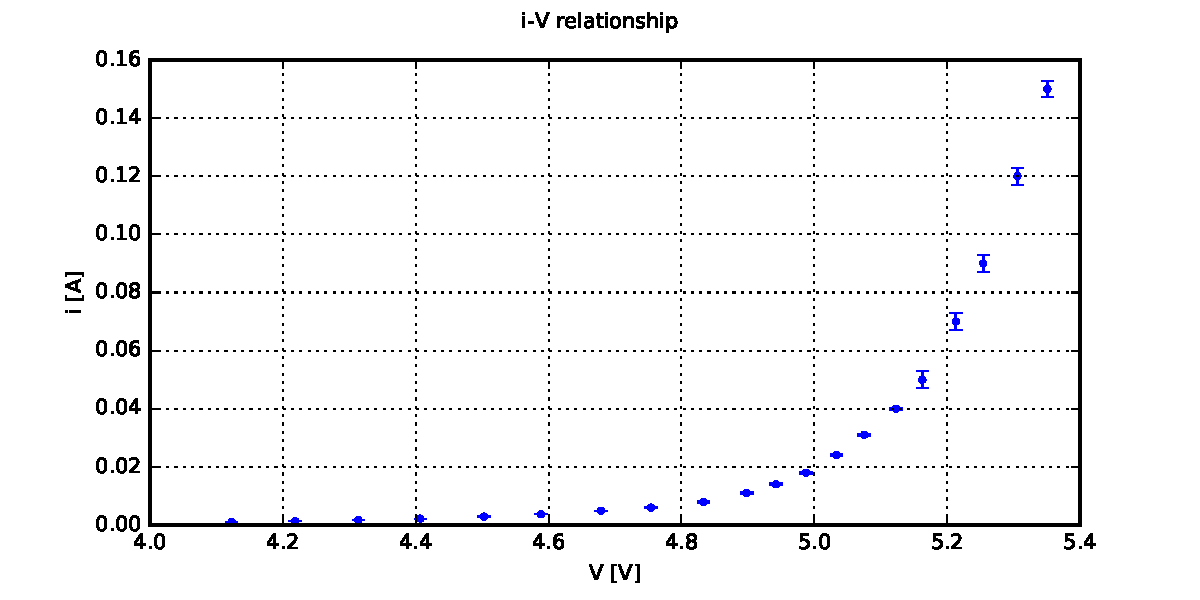
\includegraphics[width=\textwidth]{fig1Z.pdf} 
        \caption{Grafico esponenziale di $i$ in funzione di $\Delta V$}
        \label{fig:gZe}
    \end{minipage}\hfill
    \begin{minipage}{0.5\textwidth}
        \centering
        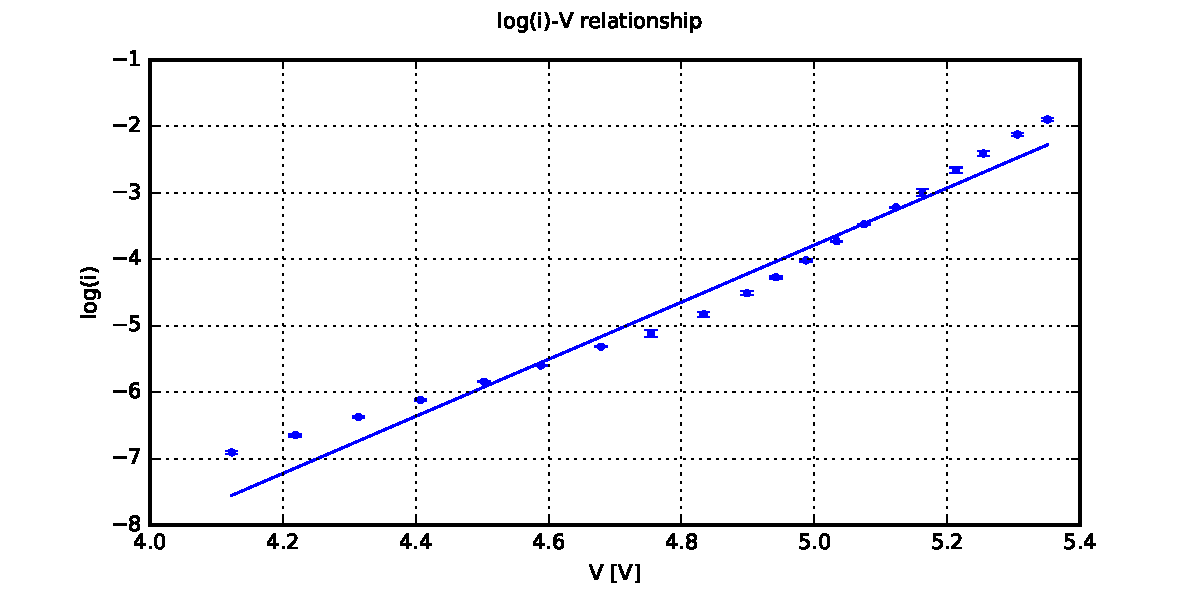
\includegraphics[width=\textwidth]{fig2Z.pdf} 
        \caption{Grafico linearizzato di $\ln{i}$ in funzione di $\Delta V$ con relativo modello}
        \label{fig:gZl}
    \end{minipage}
\end{figure}

Si nota tuttavia che nel grafico linearizzato i valori non risultano compatibili. In particolare sono rappresentate due semirette, spezzate in concomitanza del punto numero 9 della serie. Si suppone che in quel particolare punto sia successo qualcosa, plausibilmente è stato toccato il circuito e ciò ha provocato una variazione dei parametri. Si cercano quindi due nuovi modelli in grado di descrivere l'andamento dei punti prima e dopo questo punto. I nuovi parametri che si ottengono sono A1 e B1 per il primo tratto e A2 e B2 per il secondo. Li calcoliamo sempre allo stesso modo, per cui nuovamente inseriamo qui solo i risultati numerici finali.

\begin{gather}
    B_1 = 2.91 \quad A_1 = -18.9 \quad \sigma[B_1] = 0.08 \quad \sigma[A_1] = 0.5
    \\
    B_2 = 5.8 \quad A_2 = -32 \quad \sigma[B_2] = 0.2 \quad \sigma[A_2] = 1
    \\
    \label{eq:regr2}
\end{gather}

\begin{figure} [h!]
    \centering
    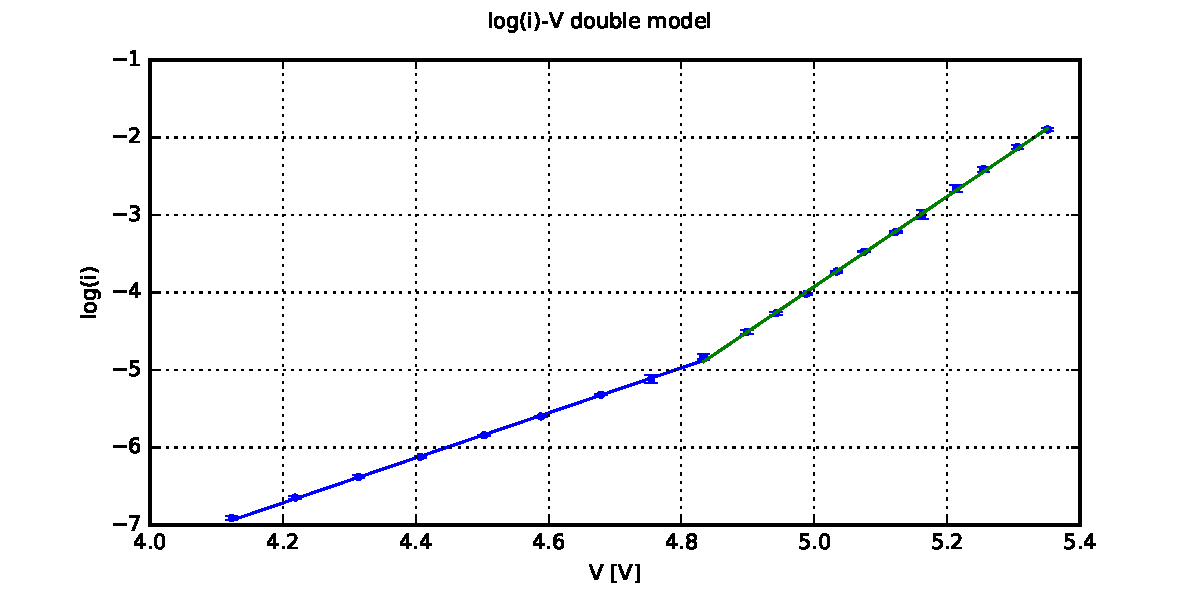
\includegraphics[width=\textwidth]{fig3Z.pdf} 
    \caption{Grafico di $\ln{i}$ in funzione di $\Delta V$ con i due modelli}
    \label{fig:gZc}
\end{figure}

Inseriamo quindi i nuovi valori all'interno di un grafico e osserviamo che questi due modelli descrivono alla perfezione i dati ottenuti nelle rispettive metà. Ciò avvalora dunque la tesi che effettuando la misura del punto 9 ci sia stata una modifica del circuito. Il grafico che otteniamo è \ref{fig:gZc}. \\ \\


Passiamo ora allo studio della resistenza dinamica. Essa rappresenta un valore tipico del diodo Zener che si modifica a seconda della corrente che scorre attraverso di esso ed alla differenza di potenziale a cui è sottoposto. Abbiamo in particolare deciso di studiare il suo comportamento in funzione della corrente. Otteniamo una curva che ha la forma di un'esponenziale. Per esserne certi consideriamo il logaritmo sia della corrente che della resistenza dinamica del nostro diodo e attraverso la regressione lineare osserviamo se ciò che otteniamo rappresenta o meno un andamento lineare. I valori che otteniamo sono i seguenti. Per quanto riguarda i risultati sulla regressione lineare non riscriviamo le formule, in quanto sempre le stesse. \\

\begin{gather}
    r_d = \frac{\Delta V}{i} \quad \sigma[r_d] = \frac{V \sigma[i]}{i^2} \quad \sigma[\ln{r_d}] = \frac{\sigma[r_d]}{r_d}
    \\
    A = -2.39 \quad B = -1.249 \quad \sigma[A] = 0.01 \quad \sigma[B] = 0.002
    \\
    \label{eq:regr3}
\end{gather}

Proviamo ad inserire quindi i risultati ottenuti nel grafico \ref{fig:gZr}, e troviamo quindi che l'andamento è rappresentato molto bene dalla retta da noi calcolata, avente i parametri sopra indicati. \\

\begin{figure} [h]
    \centering
    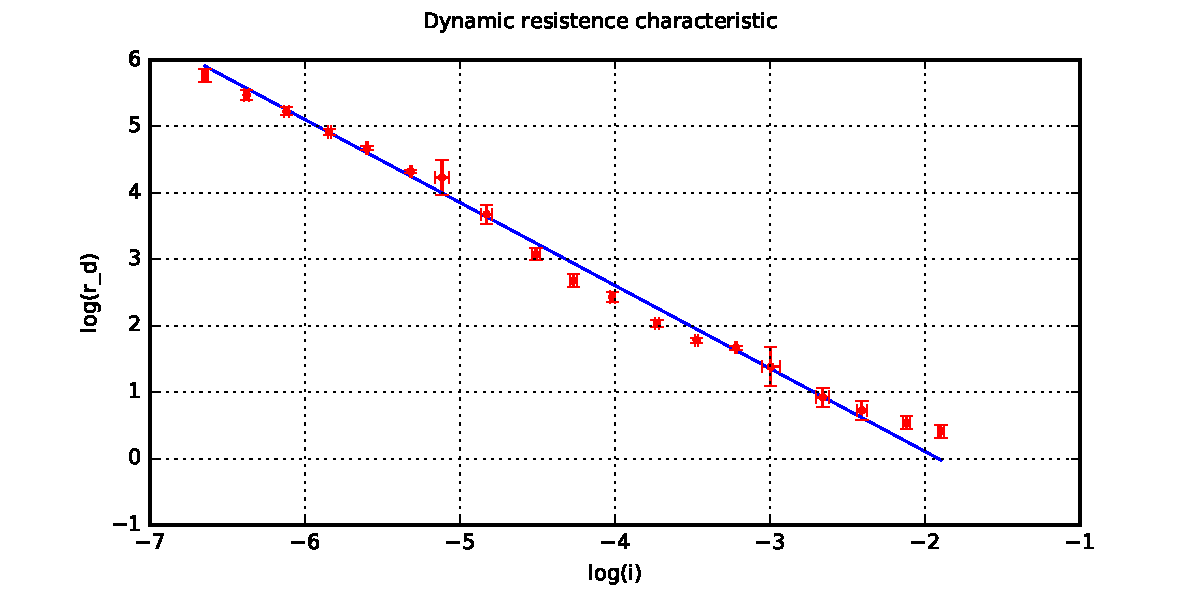
\includegraphics[width=\textwidth]{fig4Z.pdf} 
    \caption{Grafico di $\ln{r_d}$ in funzione di $\ln{i}$ con il relativo modello ottenuto tramite regressione lineare}
    \label{fig:gZr}
\end{figure}

Osserviamo inoltre che gli intervalli di incertezza di tutti i punti rientrano in almeno 3$\sigma$ dalla retta calcolata, per cui possiamo dire che effettivamente l'andamento da noi ottenuto risulta corretto. 

\subsection{Ponte di Graetz} 

Verr\'a prima preso in esame il ponte di graetz come rettificatore a doppia semionda filtrato ma senza stabilizzatore a diodo zener in fig \ref{fig:bridge}.

\begin{figure}[h]
\begin{center}
	\begin{circuitikz} []
	\draw
	(0,3.05) node[transformer core](T){}
	(T.B1) to ++(0,.45) to [short,l=$\AC 7.5\, \si{\volt}_{\textrm{rms}}$] (3,3.5) to (3,3)
	(T.B2) to ++ (0,-0.45) to (3,0.5) to (3,1)
	(T.A1) to [short,l=$\AC 220\, \si{\volt}_{\textrm{rms}}$] ++ (-.5,0)
	(T.A2) to ++ (-.5,0)
	%(T.B2)+(1,0) to [open,-, l=$\AC 7.5\, \si{\volt}$] (T.B1)
	
	(2,2) to [Do] (3,3) to [Do] (4,2)
	(2,2) to [Do] (3,1) to [Do] (4,2)
	(2,2) to  (2,0.55)
	(2,0.45) to (2,0) to (5,0)
	(4,0) node[ground] {}
	(4,2) to (5,2) to [eC,l=C] (5,0)
	(5,2) to (6,2) to [R, l=$R_l$] (6,0) to (5,0) 
	(6,2) to (7,2) to [open, -*] (7,2) node[right] {$V_{out}$}
	
	;
	\end{circuitikz}
\end{center}
\caption{Ponte di Graetz con filtro capacitivo.}
\label{fig:bridge}
\end{figure}

Il condensatore elettrolitico scelto $C=220\ \si{\micro\farad}$ ha lo scopo di stabilizzare la doppia semionda in uscita dal ponte risultando nell'onda in fig \ref{fig:brid_cfilter}.

\begin{figure}[h]
\centering
% TODO: substitute the image asking to someone for data
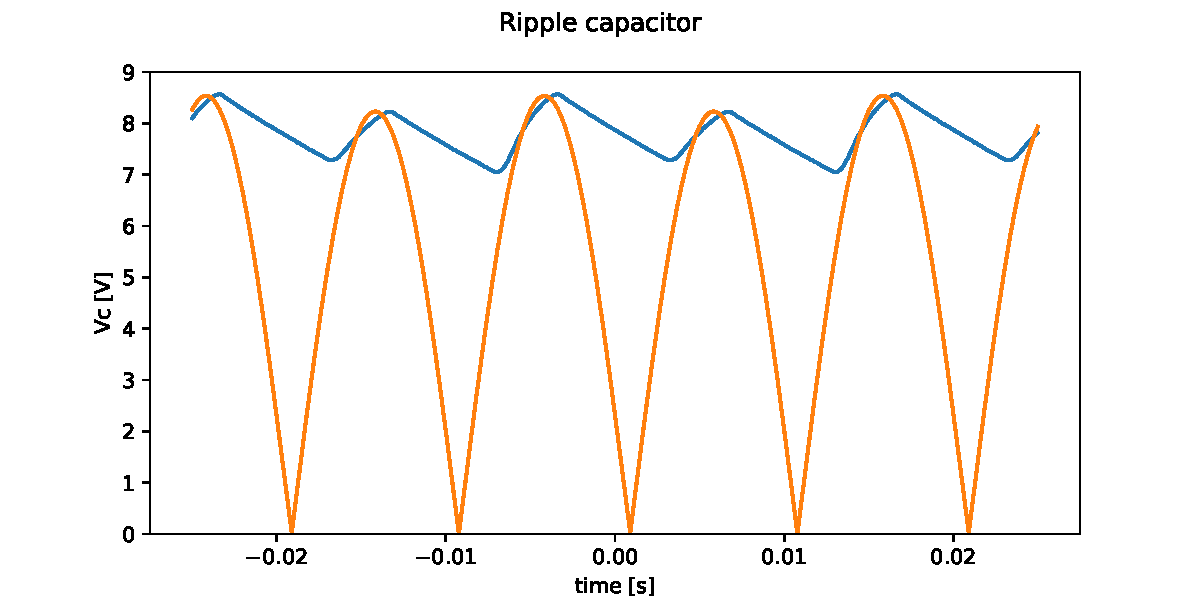
\includegraphics[width=\textwidth]{cripplefilter.pdf}
\caption{In blu la forma d'onda in uscita con il condensatore ($Rl=200\ \si{\ohm}$) ed in arancione se esso non ci fosse (quest'ultima forma d'onda \'e stata generata numericamente non potendole osservare contemporaneamente)}
\label{fig:brid_cfilter}
\end{figure}

Si pu\'o procedere a calcolare ora la massima ddp che otterrei in funzione della resistenza di carico applicata e la si confronta con i valori misurati in fig. \ref{fig:vmaxcconf}. La corrente sul carico $i_l$ \'e stata calcolata dalla $V_{out}$ misurata.

\begin{gather}
	i_{l\, max} = \frac{V_{out\, max}}{R_l} \\
	V_{out\, max} = V_{in\, max} - 2 V_d(i_{l\, max}) 
\end{gather}

\begin{figure}[h]
\centering
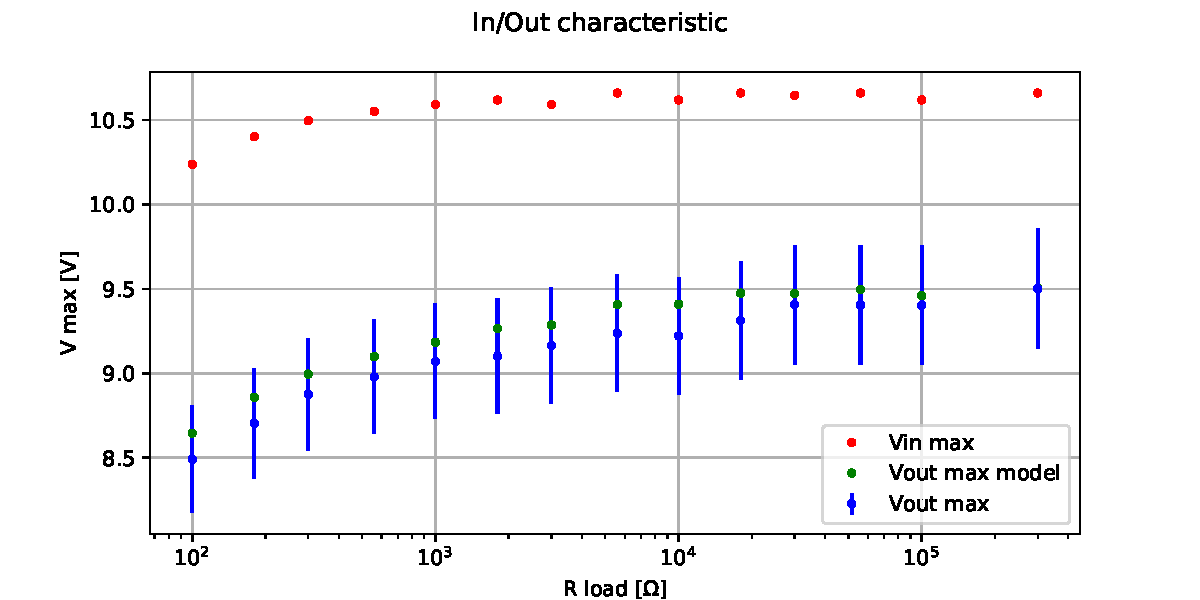
\includegraphics[width=\textwidth]{fig1.pdf}
\caption{$Vin$ misurata prima del ponte a diodi e $Vout$ misurata ai capi del carico}
\label{fig:vmaxcconf}
\end{figure}

Come si pu\'o vedere la presenza dei diodi provoca effettivamente un calo di tensione come ci si aspetta e anche l'andamento in funzione del carico \'e quello previsto.

Il ripple invece e mostrato in fig. \ref{fig:vppcconf}.

\begin{gather}
	V_{out\, pp} = \frac{i_{l\, max}}{2 f C}
\end{gather}

\begin{figure}[h]
\centering
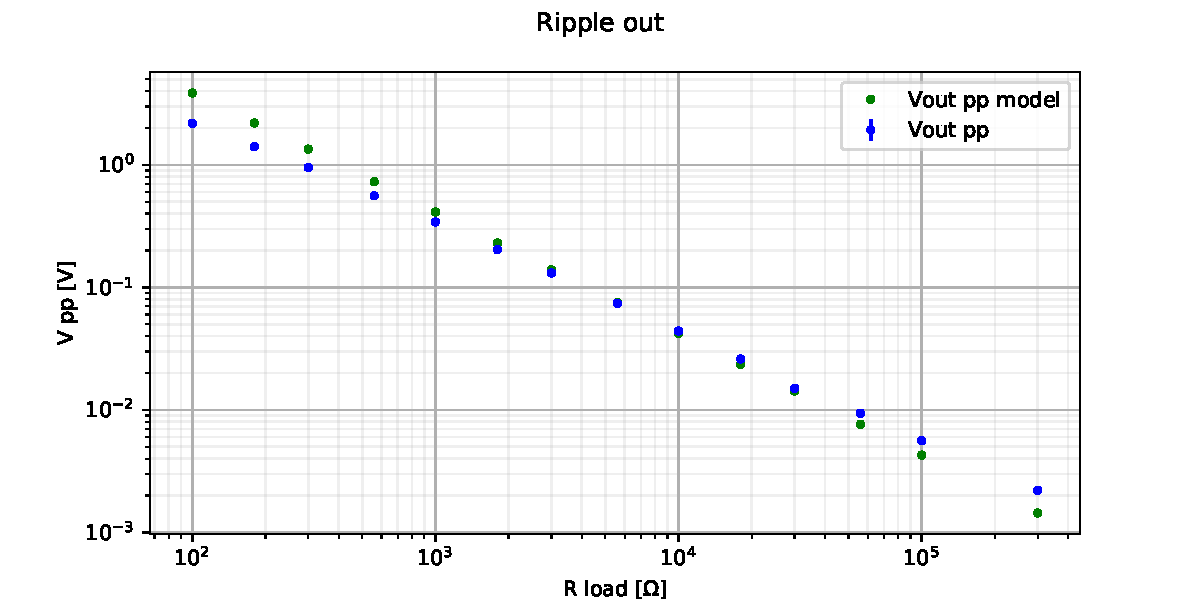
\includegraphics[width=\textwidth]{fig2.pdf}
\caption{Ripple su $Vout$ misurata ai capi del carico}
\label{fig:vppcconf}
\end{figure}

Il ripple sul condensatore segue qualitativamente l'andamento previsto e risulta del tutto compatibile per un range di carichi da $R_l=2\ \si{\kilo\ohm}$ a $R_l=30\ \si{\kilo\ohm}$.

\FloatBarrier
\newpage

Si aggiunge quindi ora il diodo zener per stabilizzare ulteriormente l'uscita secondo il circuito in figura \ref{fig:bridgez}.

\begin{figure}[h]
\begin{center}
	\begin{circuitikz} []
	\draw
	(0,3.05) node[transformer core](T){}
	(T.B1) to ++(0,.45) to [short,l=$\AC 7.5\, \si{\volt}_{\textrm{rms}}$] (3,3.5) to (3,3)
	(T.B2) to ++ (0,-0.45) to (3,0.5) to (3,1)
	(T.A1) to [short,l=$\AC 220\, \si{\volt}_{\textrm{rms}}$] ++ (-.5,0)
	(T.A2) to ++ (-.5,0)
	%(T.B2)+(1,0) to [open,-, l=$\AC 7.5\, \si{\volt}$] (T.B1)
	
	(2,2) to [Do] (3,3) to [Do] (4,2)
	(2,2) to [Do] (3,1) to [Do] (4,2)
	(2,2) to  (2,0.55)
	(2,0.45) to (2,0) to (5,0)
	(4,0) node[ground] {}
	(4,2) to (5,2) to [eC,l=C] (5,0)
	(5,2) to [R,l=R,i>_=$i_R$] (7,2) to [zzDo,invert,i>_=$i_z$] (7,0)
	(7,2) to (8,2) to [R, l=$R_l$,i>_=$i_l$] (8,0) to (5,0) 
	(8,2) to (9,2) to [open, -*] (9,2) node[right] {$V_{out}$}
	(5,2) to (5,3) to (9,3) to [open, -*] (9,3) node[right] {$V_c$}
	
	;
	\end{circuitikz}
\end{center}
\caption{Ponte di Graetz con filtro capacitivo e diodo zener.}
\label{fig:bridgez}
\end{figure}

In questa configurazione il diodo svolge la funzione di diminuire il ripple (fig. \ref{fig:ripplecomp}) che si era visto con solamente il condensatore al costo di dissipare potenza nella resistenza $R$ e nello zener.

\begin{figure}[h]
\centering
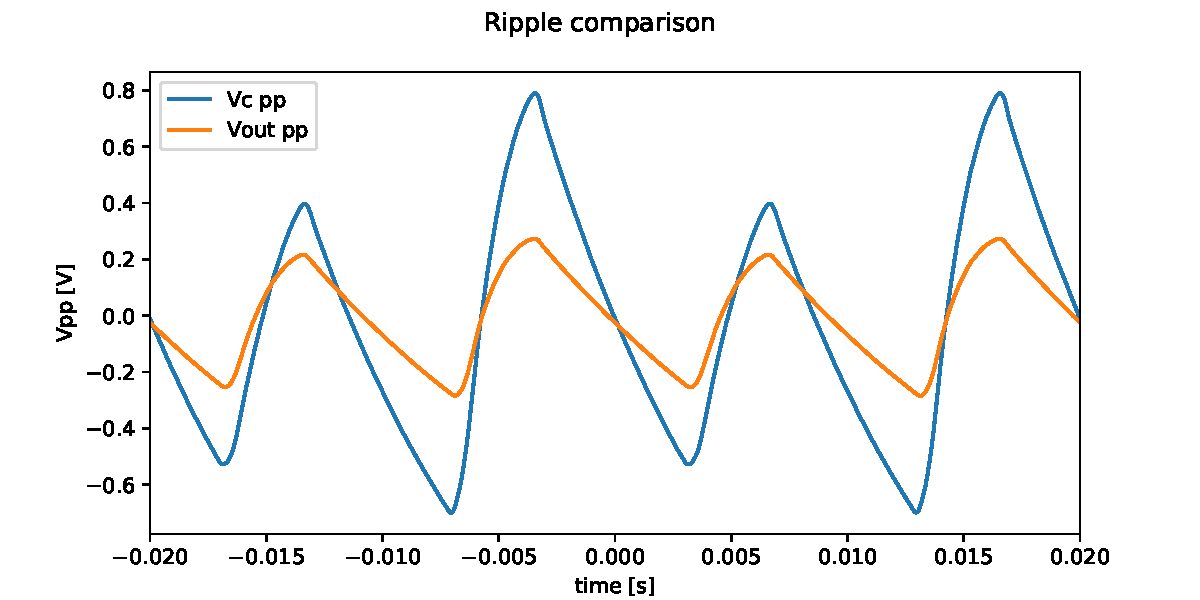
\includegraphics[width=\textwidth]{ripplecomp.pdf}
\caption{Confronto ripple con $R_l = 200 \ \si{\ohm}$.}
\label{fig:ripplecomp}
\end{figure}

Chiamata $i_z(V_z)$ la caratteristica tensione-corrente dello zener ed utilizzando la $V_{out}$ misurata per il calcolo di $i_l$ e $i_z$ si pu\'o definire:

\begin{gather}
	i_{l\, max} = \frac{V_{out\, max}}{R_l} \\
	i_{z\, max} = i_z(V_{out\, max}) \\
	i_{R\, max} = i_{z\, max} + i_{out\, max} \\
	V_{out\, max} = V_{c\, max} - i_{R\, max} R
\end{gather}

\begin{figure}[h]
\centering
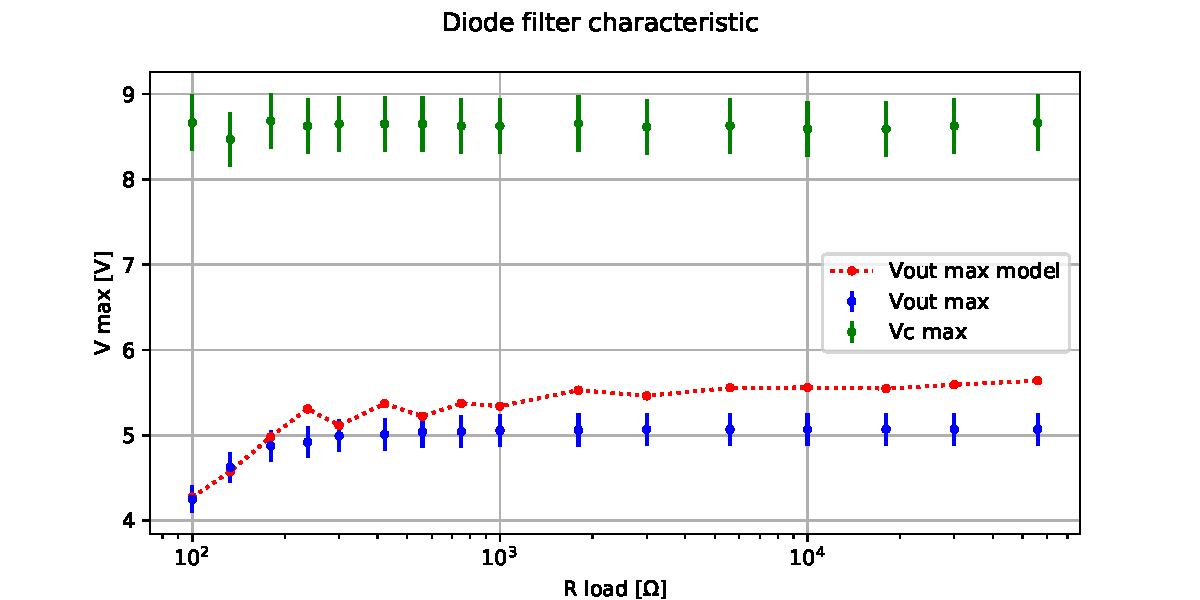
\includegraphics[width=\textwidth]{fig4.pdf}
\caption{$V_{out}$ in funzione del carico}
\label{fig:vdiod}
\end{figure}

Come si pu\'o vedere la presenza dello stadio ulteriore di filtraggio diminuisce l'output del circuito.

Considerata $r_z(i_z)$ la resistenza dinamica del diodo, il ripple viene stimato in questo modo:

\begin{gather}
	V_{c\, pp} = \frac{i_{R\, max}}{2fC} \\
	V_{out\, pp} = V_{c\, pp} \frac{r_z}{r_z+R(1+\frac{r_z}{R_l})}
\end{gather}

\begin{figure}[h]
\centering
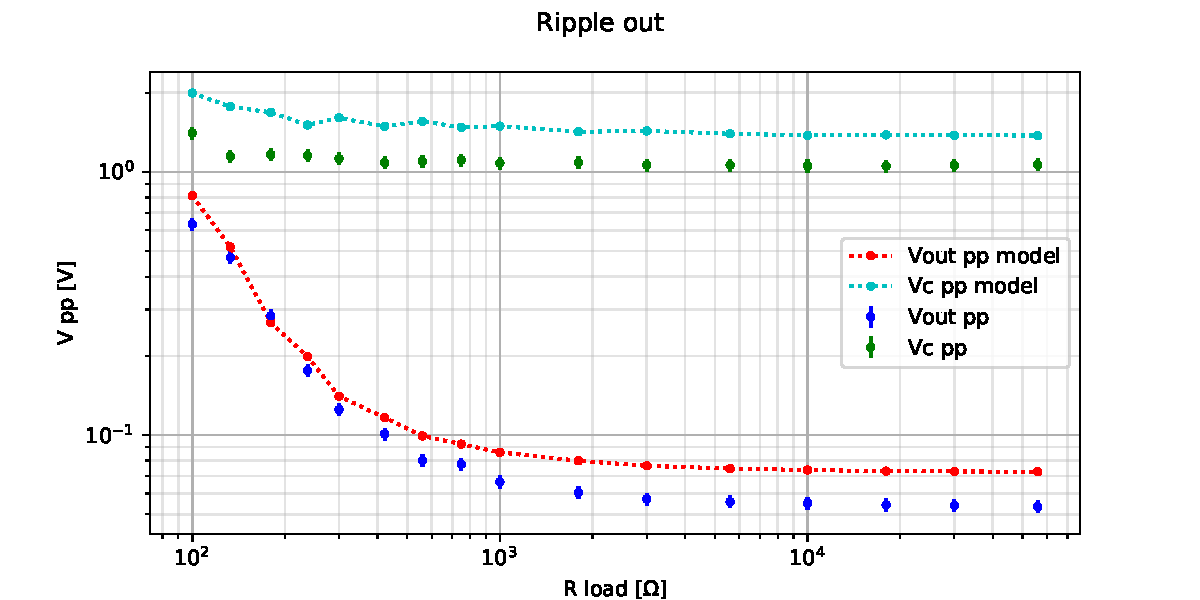
\includegraphics[width=\textwidth]{fig5.pdf}
\caption{Ripple in funzione del carico}
\label{fig:vdiodpp}
\end{figure}











\newpage

\section{Conclusioni}
In conclusione i diodi mostrano effettivamente l'andamento esponenziale in corrente-tensione tipico di una giunzione P-N.
La loro applicazione nel ponte di Graetz \'e di incalcolabile utilit\'a nel mondo moderno in cui tutta l'elettronica che abbiamo a disposizione funziona in tensioni continue mentre la tensione di rete \'e alternata.
Per il filtraggio il solo condensatore fornisce l'efficienza massima essendo ovviamente un componente solo reattivo a discapito di accettare un ripple in uscita. Questo tipo di compromesso pu\'o essere accettabile in molte applicazioni come ad esempio in entrata ad un ulteriore stadio di filtraggio per poi ottenere un'uscita pi\'u pulita oppure per il driving di componenti come motori DC o illuminazione.
L'utilizzo di un diodo Zener fornisce effettivamente gli effetti voluti ma il suo impiego risulta effettivo solamente se il carico non richiede troppa corrente. Per questo motivo \'e realmente impiegato solo come ultimo stadio di alimentazione per sensoristica ecc. In tutti gli altri casi si preferisce un buck converter per la sua elevata efficienza e scalabilit\'a.

\end{document}
